\section{Data Driven Background Estimation Methods}
\label{sec:datadriven}
We have developed two data-driven methods to 
estimate the background in the signal region.
The first one exploits the fact that 
\Ht\ and $y$ are nearly 
uncorrelated for the $t\bar{t}$ background 
(Section~\ref{sec:abcd});  the second one 
is based on the fact that in $t\bar{t}$ the
$P_T$ of the dilepton pair is on average 
nearly the same as the $P_T$ of the pair of neutrinos
from $W$-decays, which is reconstructed as \met\ in the
detector.

We study the closure of these methods using our madgraph \ttbar\ sample, as well as 
the powheg sample TTTo2L2Nu2B\_7TeV-powheg-pythia6\_Spring11-PU\_S1\_START311\_V1G1-v1
which has approximately 10 times more events in the dilepton channel than the madgraph sample.
We use these samples to estimate correction factors and systematic uncertainties for the background predictions. 
However, the final choice of correction factors and uncertainties will be extracted from the Summer11 \ttbar\ madgraph
sample which will have 50 times as many events as the current madgraph sample. 
For these studies, we do not apply trigger efficiency corrections or reweighting for
number of reconstructed vertices since are not comparing MC to data. 

\subsection{ABCD method}
\label{sec:abcd}


\begin{figure}[hbt]
\begin{center}
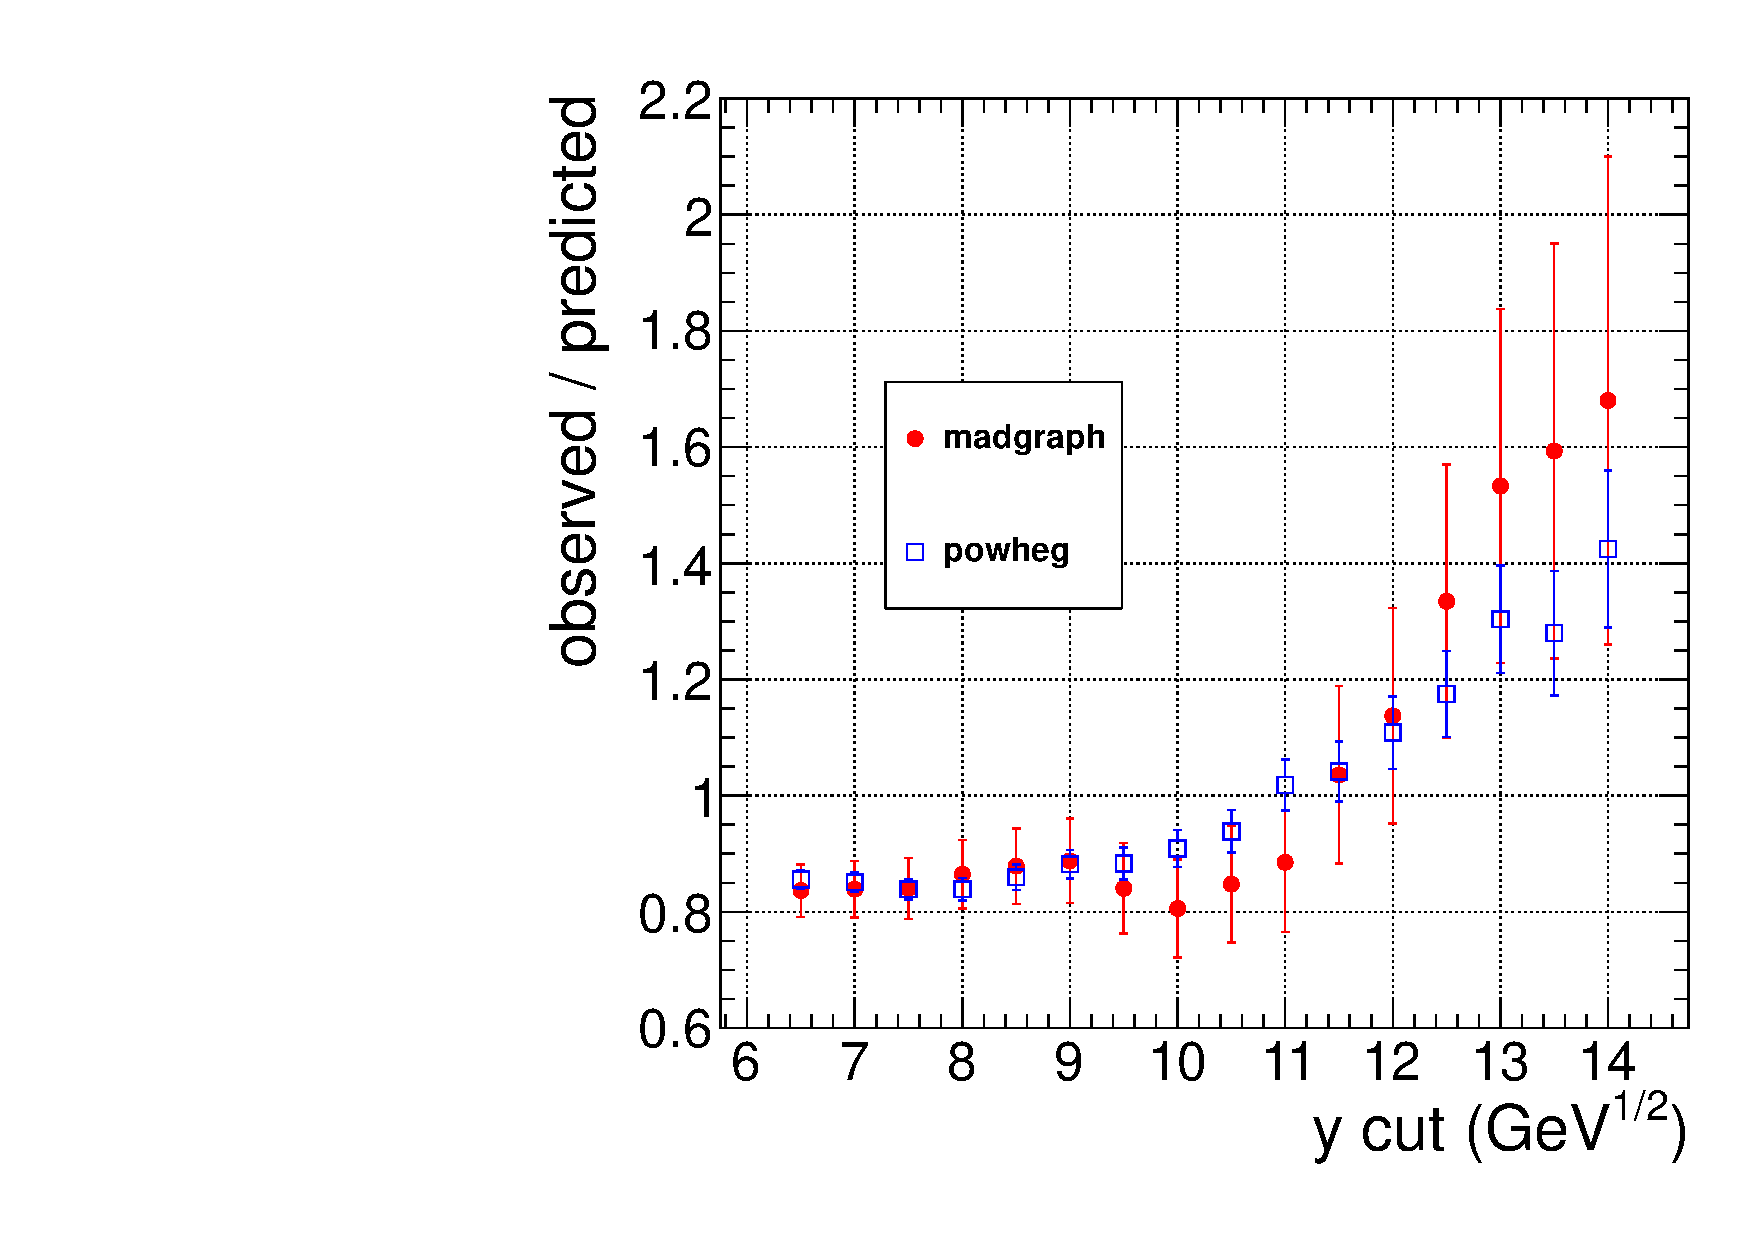
\includegraphics[width=0.48\linewidth]{plots/abcd_y.pdf}
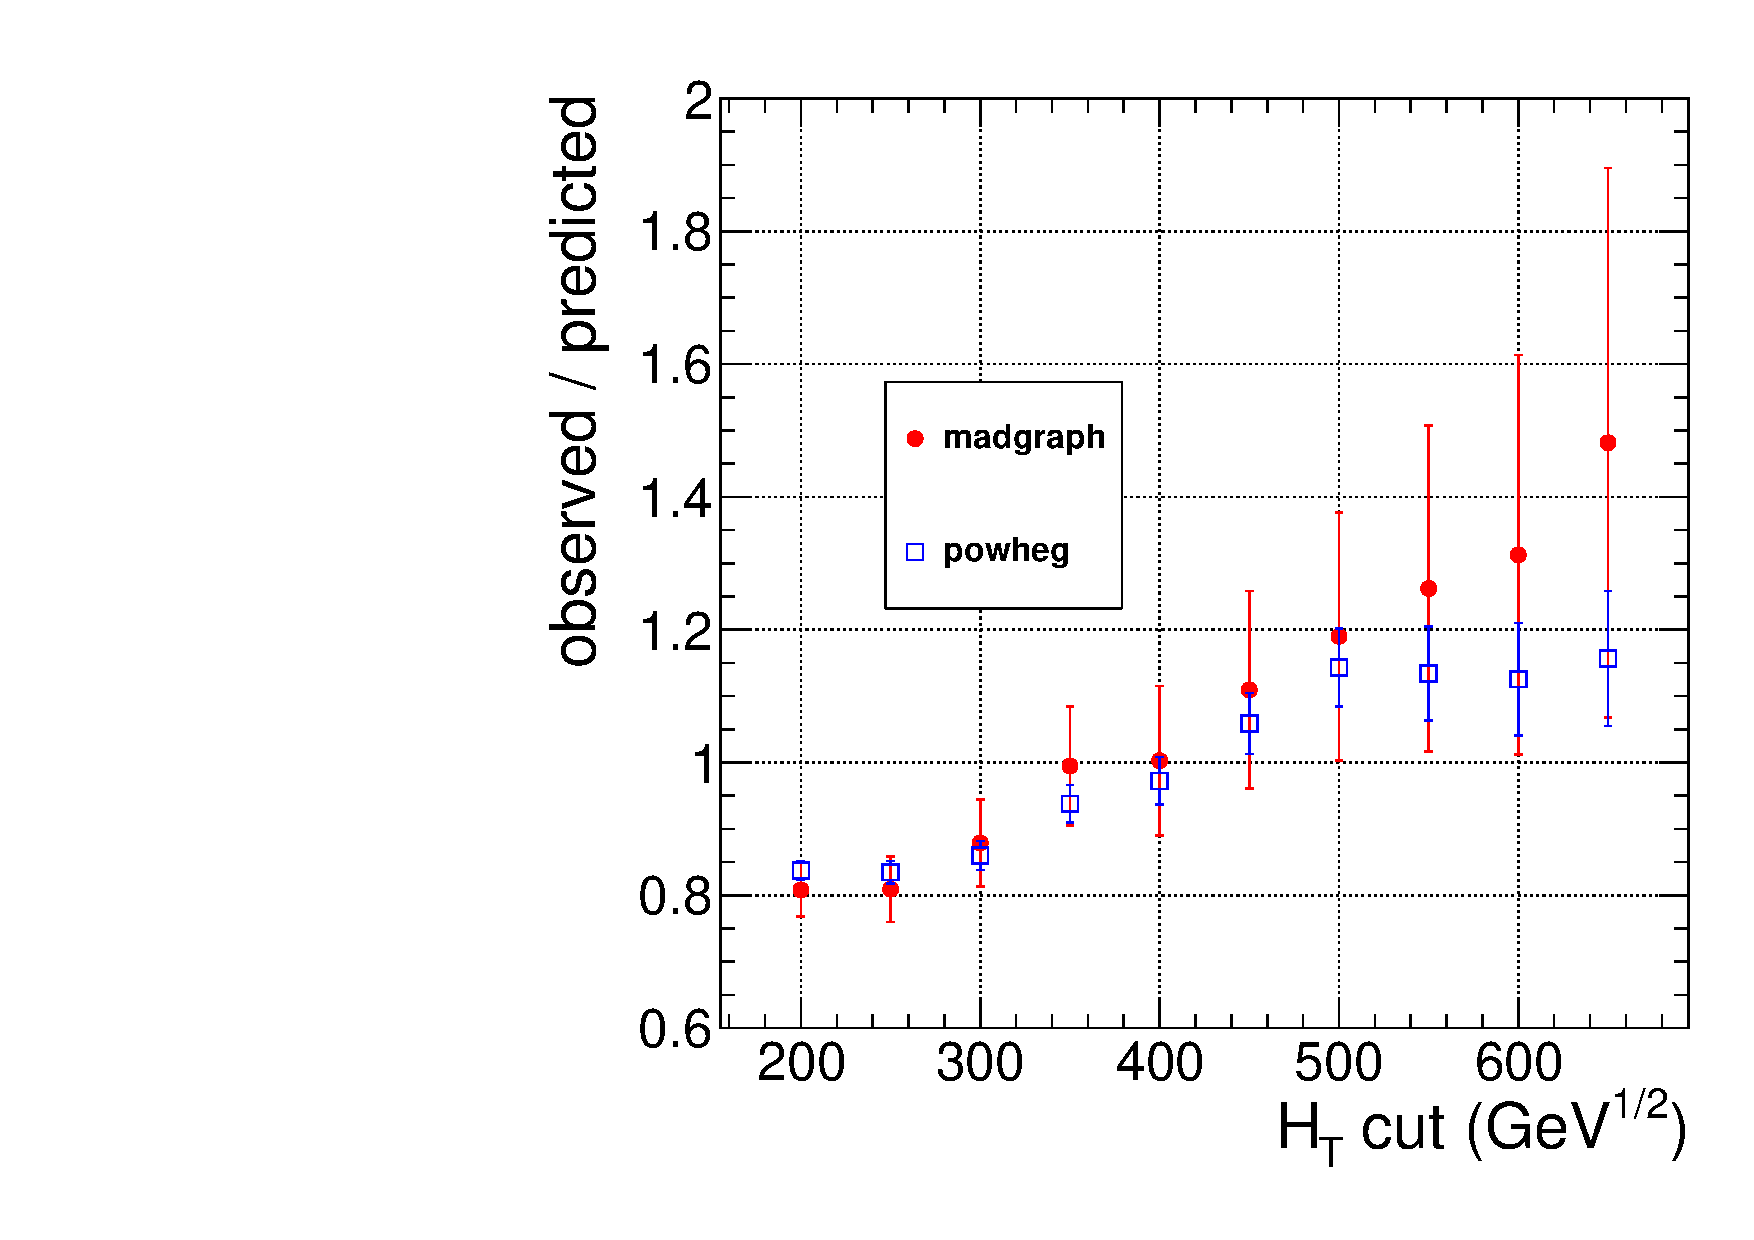
\includegraphics[width=0.48\linewidth]{plots/abcd_ht.pdf}
\caption{\label{fig:victory}\protect Variation of observed/predicted
for the ABCD method as a function of the $y$ and \Ht\ cuts defining
the signal region.}
\end{center}
\end{figure}


We find that in $t\bar{t}$ events \Ht\ and 
$y$ are nearly uncorrelated, 
as demonstrated in Fig.~\ref{fig:uncor}.
Thus, we can use an ABCD method in the $y$ vs. \Ht
plane to estimate the background in a data driven way. We dfine 4 regions in the 
plane of $y$ vs. \Ht, as shown in Figs.~\ref{abcdData1}-\ref{abcdData2}.
The region D is the signal region, and the regions A, B and C are control regions.
The predicted background in region D is given by $N_A \times N_C / N_B$.

In Table~\ref{tab:mcabcd}, we quote the MC expected yields for 1~fb$^{-1}$. In
general we find that the prediction agrees with the observed signal yield within
$\sim$30-50\% for all signal regions. Based on these results, we apply the
scale factors and uncertainties summarized in Table~\ref{tab:cor} to the
predicted background from the ABCD method.


\begin{table}[hbt]
\begin{center}
\caption{\label{tab:mcabcd} Expected yields in 1~fb$^{-1}$ in the four
ABCD regions (depicted in Figs.~\ref{abcdData1}-\ref{abcdData2},
as well as the predicted yield in region D given
by A $\times$ C / B and the ratio of the observed signal yield to the prediction. The quoted uncertainties are statistical
only, assuming Gaussian errors.
}
\begin{tabular}{lcccccccc}
\hline
signal region &           sample  &                A  &                B  &                C  &                D  &   A $\times$ B / C   & obs/pred\\
\hline

\hline

2010 signal region      &   madgraph  & 251.3  $\pm$  6.1  &951.5  $\pm$  11.9  & 165.2  $\pm$  4.9  & 38.3  $\pm$  2.4  & 43.6  $\pm$  1.8  &0.88  $\pm$  0.07 \\
                        &   powheg    & 231.7  $\pm$  2.0  &850.6  $\pm$  3.7   & 157.8  $\pm$  1.6  & 37.0  $\pm$  0.8  & 43.0  $\pm$  0.6  &0.86  $\pm$  0.02 \\

\hline

high $y$ signal region  &   madgraph  & 18.4  $\pm$  1.6   &951.5  $\pm$  11.9  & 165.2  $\pm$  4.9  &  4.9  $\pm$  0.9  &  3.2  $\pm$  0.3  &1.53  $\pm$  0.30 \\
                        &     powheg  & 17.3  $\pm$  0.5   &850.6  $\pm$  3.7   & 157.8  $\pm$  1.6  &  4.2  $\pm$  0.3  &  3.2  $\pm$  0.1  &1.30  $\pm$  0.09 \\

\hline

high \Ht\ signal region &   madgraph  & 251.3  $\pm$  6.1  &951.5  $\pm$  11.9  & 11.1  $\pm$  1.3  &  3.8  $\pm$  0.8  &  2.9  $\pm$  0.3  &1.31  $\pm$  0.30 \\
                        &     powheg  & 231.7  $\pm$  2.0  &850.6  $\pm$  3.7   & 12.5  $\pm$  0.5  &  3.8  $\pm$  0.3  &  3.4  $\pm$  0.1  &1.13  $\pm$  0.08 \\


\hline
%high $y$ signal region  & 

\hline
\end{tabular}
\end{center}
\end{table}


\begin{table}[hbt]
\begin{center}
\caption{\label{tab:cor} 
}
\begin{tabular}{lcc}
\hline
signal region               &           ABCD  &                \ptll  \\
\hline
2010 signal region          &   $1.0 \pm 0.2$ &        $1.4 \pm 0.2$   \\
high $y$  signal region     &   $1.3 \pm 0.3$ &        $1.7 \pm 0.3$   \\
high \Ht\ signal region     &   $1.2 \pm 0.2$ &        $1.3 \pm 0.2$   \\
\hline
\end{tabular}
\end{center}
\end{table}


\clearpage

\subsection{Dilepton $P_T$ method}
\label{sec:victory}
This method is based on a suggestion by V. Pavlunin\cite{ref:victory},
and was investigated by our group in 2009\cite{ref:ourvictory}.
The idea is that in dilepton $t\bar{t}$ events the lepton and neutrinos
from $W$ decays have the same $P_T$ spectrum (modulo $W$ polarization 
effects).  One can then use the observed 
$P_T(\ell\ell)$ distribution to model the sum of neutrino $P_T$'s which 
is identified with the \met.

Then, in order to predict the $t\bar{t} \to$ dilepton contribution to a 
selection with \met$+$X, one applies a cut on $P_T(\ell\ell)+$X instead.
In practice one has to rescale the result of the $P_T(\ell\ell)+$X selection
to account for the fact that any dilepton selection must include a 
moderate \met cut in order to reduce Drell Yan backgrounds.  This 
is discussed in Section 5.3 of Reference~\cite{ref:ourvictory}; for a \met
cut of 50 GeV, the rescaling factor is obtained from the MC as


\begin{figure}[hbt]
\begin{center}
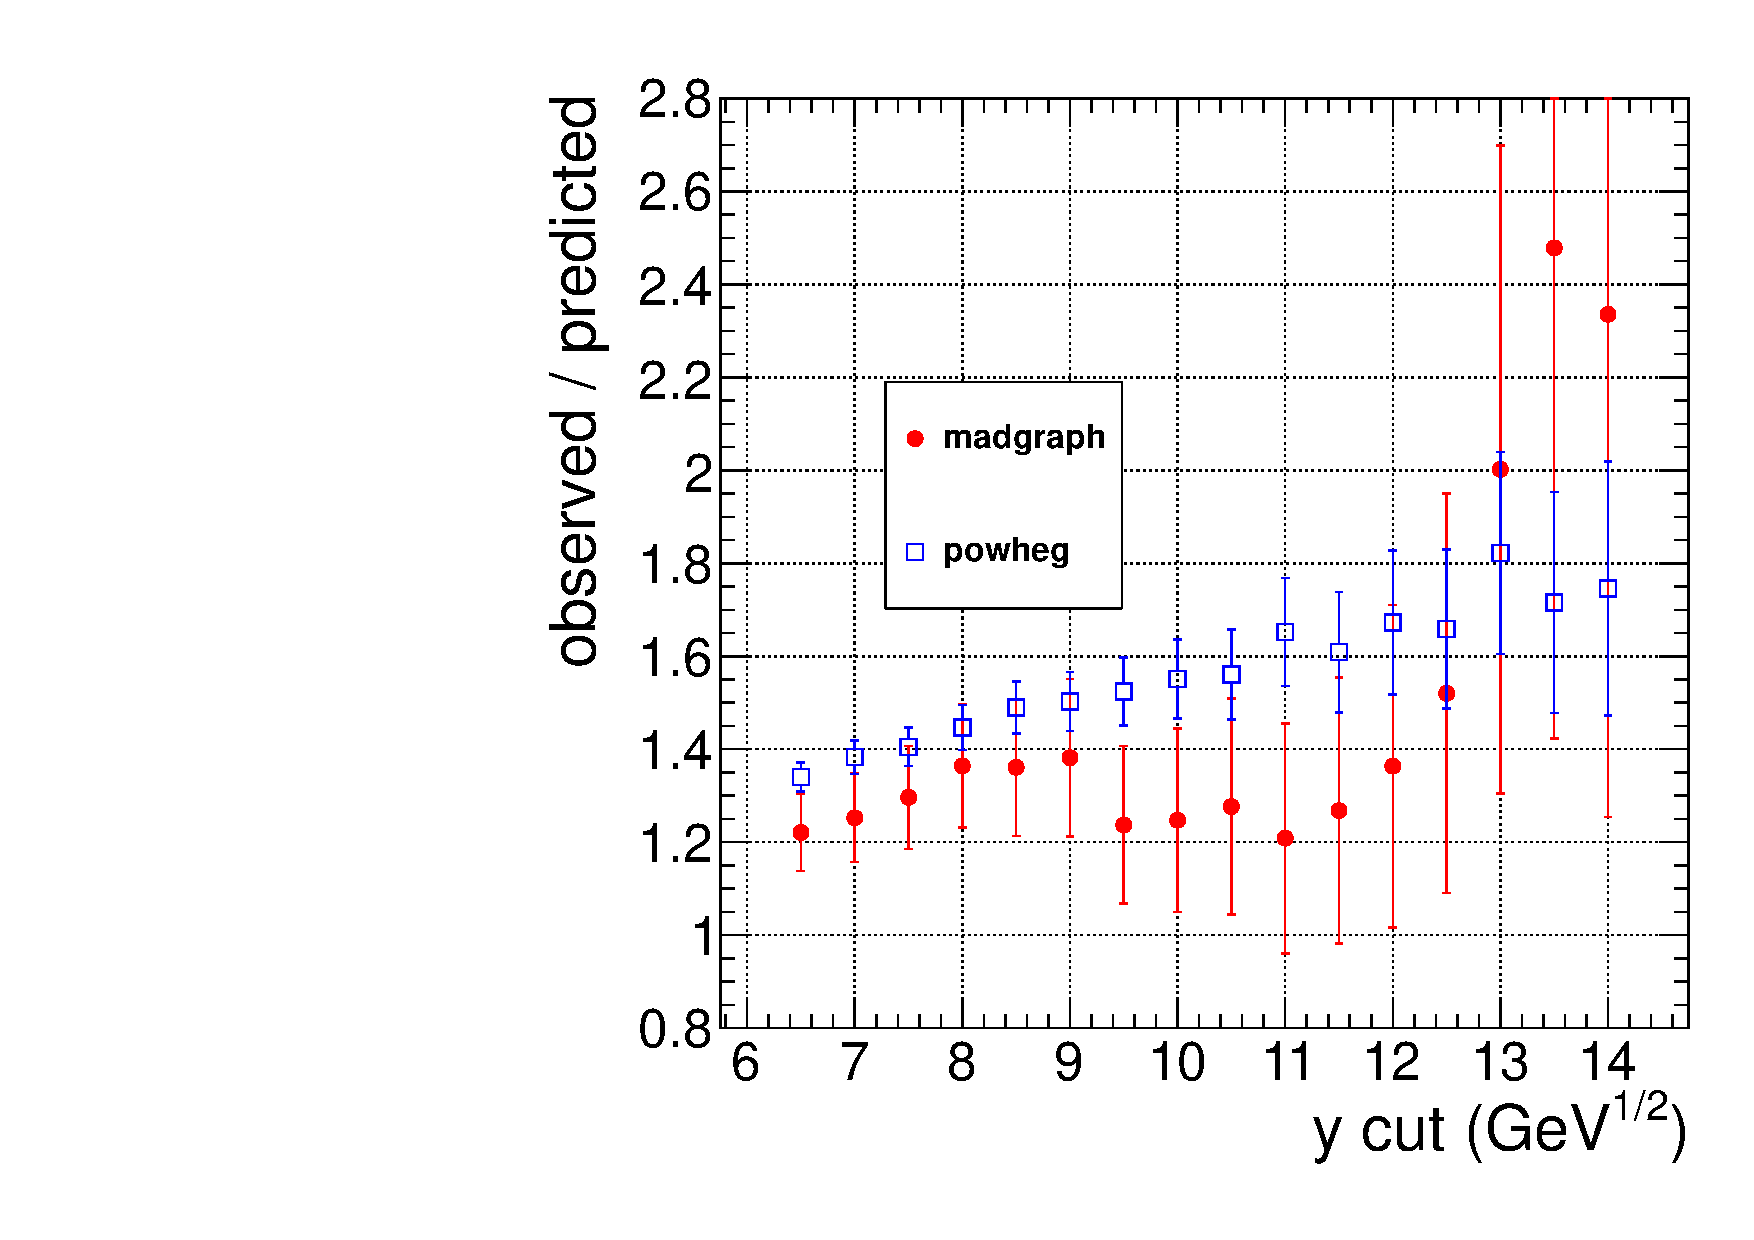
\includegraphics[width=0.48\linewidth]{plots/victory_yvary.pdf}
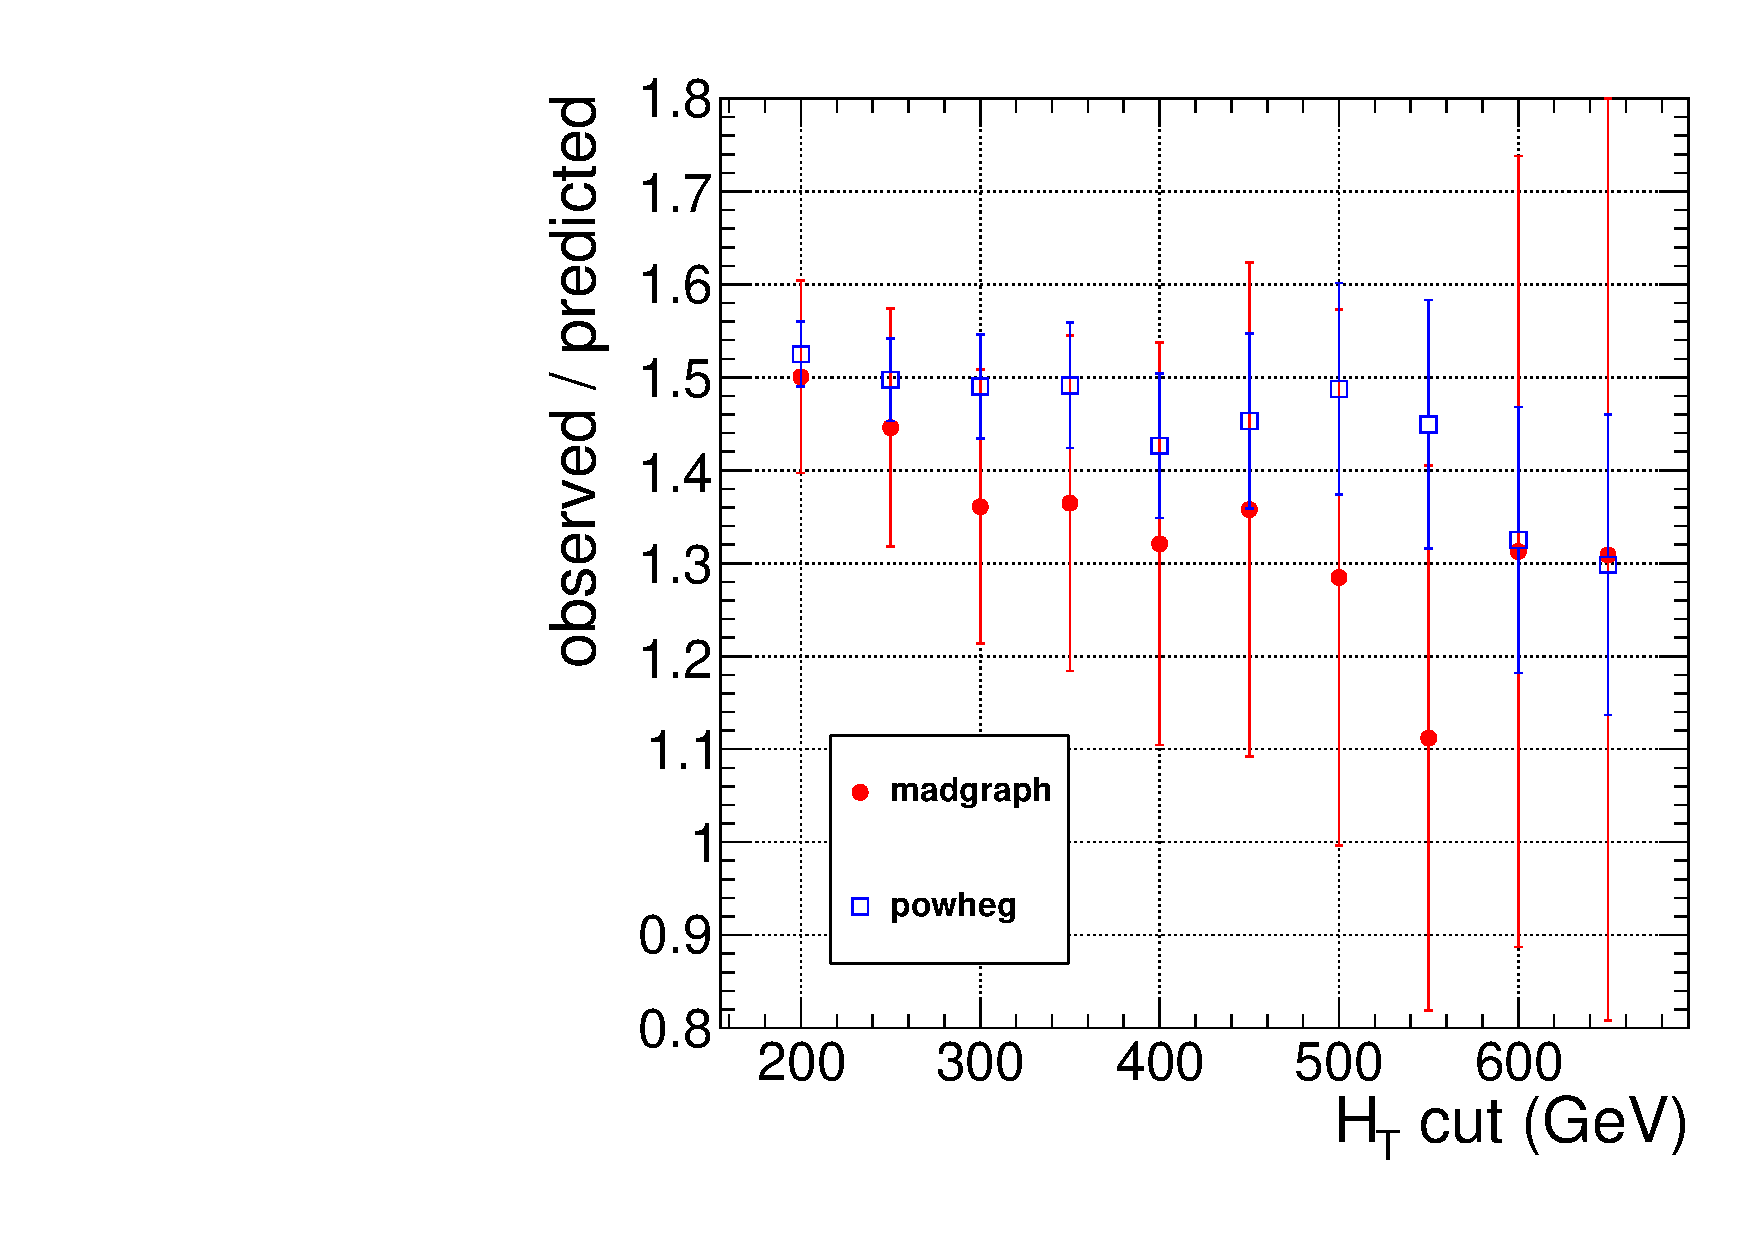
\includegraphics[width=0.48\linewidth]{plots/victory_htvary.pdf}
\caption{\label{fig:victory}\protect Variation of observed/predicted
for the \ptll\ method as a function of the $y$ and \Ht\ cuts defining
the signal region.}
\end{center}
\end{figure}


\begin{table}[hbt]
\begin{center}
\caption{\label{tab:mcabcd} Expected observed and predicted yields in 1~fb$^{-1}$ for the \ptll\ method, 
and the ratio of the observed signal yield to the prediction. The quoted uncertainties are statistical
only, assuming Gaussian errors.
}
\begin{tabular}{lcccccccc}
\hline
signal region &           sample  &                predicted  &                observed  &                obs/pred   \\ 
\hline

\hline

2010 signal region      &   madgraph  & 28.2 $\pm$ 2.5   &      38.3 $\pm$ 2.4   &     1.36 $\pm$ 0.15  \\
                        &   powheg    & 24.8 $\pm$ 0.8   &      37.0 $\pm$ 0.8   &     1.49 $\pm$ 0.06  \\


\hline

high $y$ signal region  &   madgraph  & 2.4 $\pm$ 0.7   &       4.9 $\pm$ 0.9   &     2.00 $\pm$ 0.70  \\
                        &     powheg  & 2.3 $\pm$ 0.2   &       4.2 $\pm$ 0.3   &     1.82 $\pm$ 0.22  \\

\hline

high \Ht\ signal region &   madgraph  & 2.9 $\pm$ 0.8   &       3.8 $\pm$ 0.8   &     1.31 $\pm$ 0.43  \\
                        &     powheg  & 2.9 $\pm$ 0.2   &       3.8 $\pm$ 0.3   &     1.33 $\pm$ 0.14  \\


\hline
%high $y$ signal region  & 

\hline
\end{tabular}
\end{center}
\end{table}


%
\begin{center}
$ K = \frac{\int_0^{\infty} {\cal N}(\ptll)~~d\ptll~}{\int_{50}^{\infty} {\cal N}(\ptll)~~d\ptll~} = 1.5$
\end{center}

{\color{red} \bf HERE I WILL PUT THE VICTORY MC CLOSURE STUDIES FOR THE 3 SIGNAL REGIONS}

\subsection{Signal Contamination}
\label{sec:sigcont}

All data-driven methods are in principle subject to signal contaminations
in the control regions, and the methods described in 
Sections~\ref{sec:abcd} and~\ref{sec:victory} are not exceptions.
Signal contamination tends to dilute the significance of a signal
present in the data by inflating the background prediction.

It is hard to quantify how important these effects are because we 
do not know what signal may be hiding in the data.  Having two
independent methods (in addition to Monte Carlo ``dead-reckoning'')
adds redundancy because signal contamination can have different effects
in the different control regions for the two methods.
For example, in the extreme case of a
new physics signal 
with $P_T(\ell \ell) = \met$, an excess of events would be seen 
in the ABCD method but not in the $P_T(\ell \ell)$ method.


The LM points are benchmarks for SUSY analyses at CMS.  The effects
of signal contaminations for a couple such points are summarized
in Table~\ref{tab:sigcont}. Signal contamination is definitely an important
effect for these two LM points, but it does not totally hide the
presence of the signal.


\begin{table}[htb]
\begin{center}
\caption{\label{tab:sigcont} Effects of signal contamination 
for the two data-driven background estimates. The three columns give
the expected yield in the signal region and the background estimates
using the ABCD and $P_T(\ell \ell)$ methods. Results are normalized to 204~pb$^{-1}$.
{\color{red} \bf UPDATE ME }
}
\begin{tabular}{lccc}
\hline
            &      Yield      &      ABCD    & $P_T(\ell \ell)$  \\
\hline
SM only     &       1.3      &      1.3    &       0.9        \\
SM + LM1    &       9.9      &      6.1    &       2.4        \\
SM + LM3    &       4.8      &      1.8    &       1.6        \\
\hline
\end{tabular}
\end{center}
\end{table}

